\documentclass[a4paper]{scrartcl}
\begingroup\expandafter\expandafter\expandafter\endgroup
\expandafter\ifx\csname pdfsuppresswarningpagegroup\endcsname\relax
\else
  \pdfsuppresswarningpagegroup=1\relax
\fi
\usepackage[british]{babel}
\usepackage{amsmath}
\usepackage{xspace}
\usepackage{cite}
\usepackage{graphicx}
\graphicspath{ {./figs/} }
\usepackage{siunitx}
\usepackage{hyperref}

% custom commands
\newcommand{\alphas}{\ensuremath{\alpha_S}\xspace}
\newcommand{\tvar}{\ensuremath{t}\xspace}
\newcommand{\diff}{\ensuremath{\text{d}}\xspace}

% title information
\title{\alphas fit using a differential jet observable and the inclusion of
theory uncertainties by on-the-fly reweighting}
\author{Enrico Bothmann \and Luigi Del Debbio \and Nathan Hartland \and Steffen
Schumann}
\date{\today}

\begin{document}
\maketitle
\section{The azimuthal decorrelation in dijet events}
State the source of experimental data and break down its uncertainties.
\cite{Khachatryan:2011zj,Khachatryan:2016hkr}
\section{Monte Carlo predictions}
Describe the Sherpa setup used and compare LOPS, MEPS@LO, \dots\ to data.
\begin{figure}[p]
    \centering
    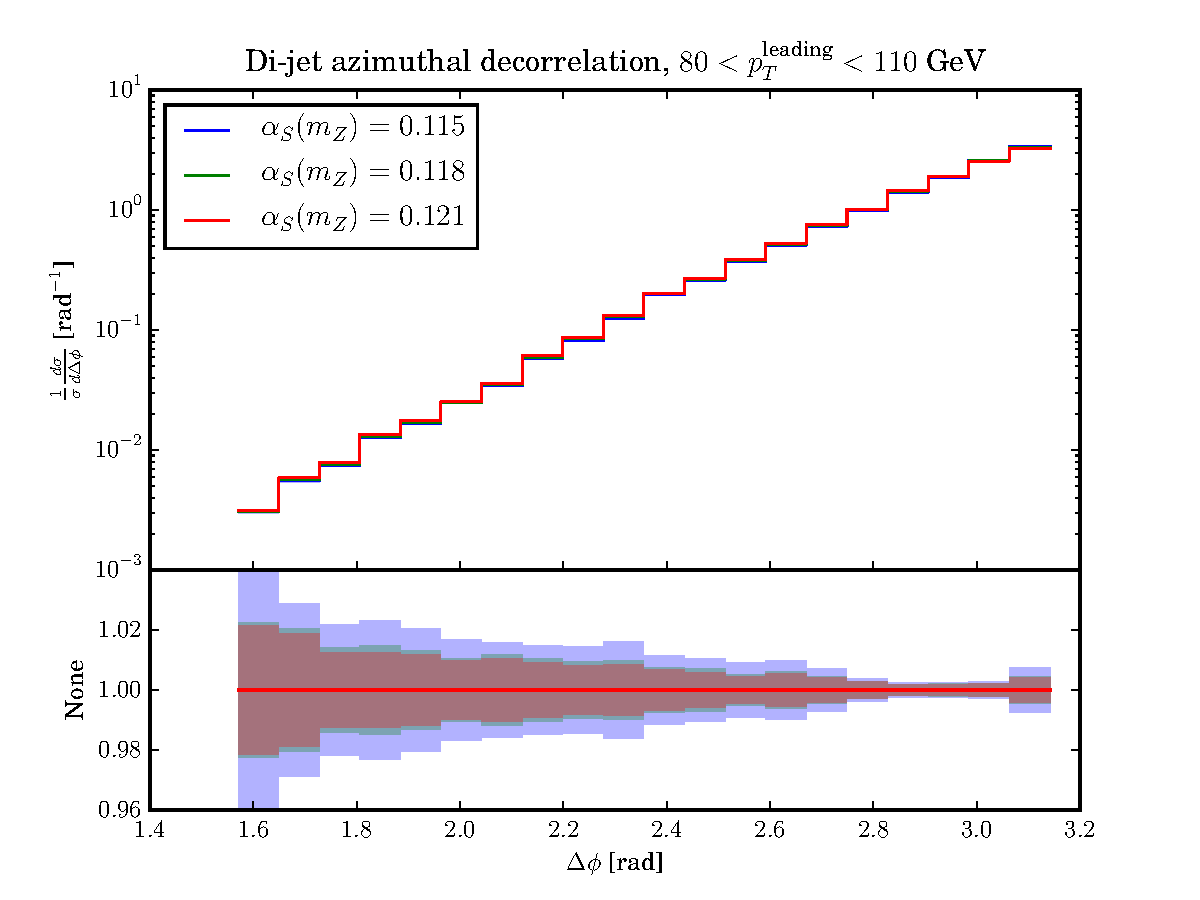
\includegraphics[width=0.49\textwidth]{d01-x01-y01_PDF-errors}
    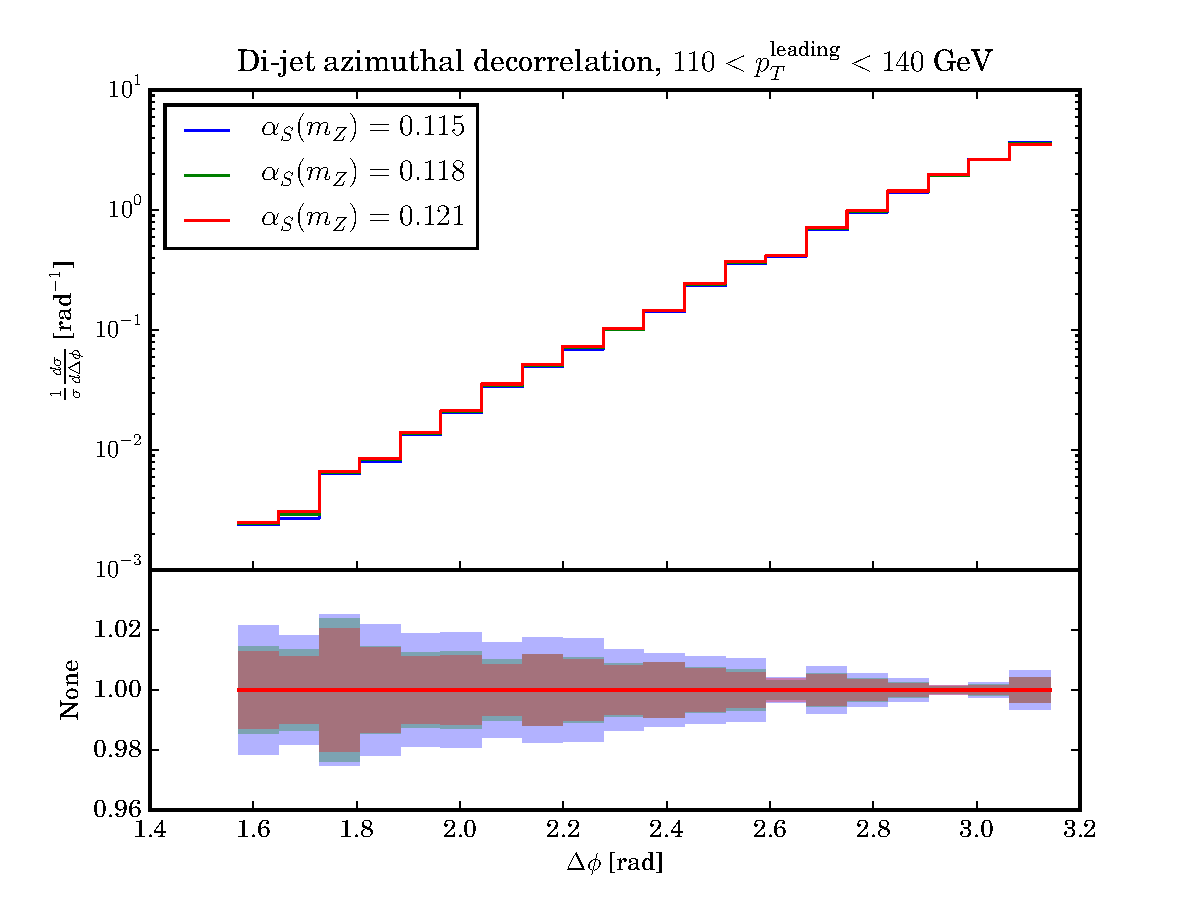
\includegraphics[width=0.49\textwidth]{d02-x01-y01_PDF-errors}
    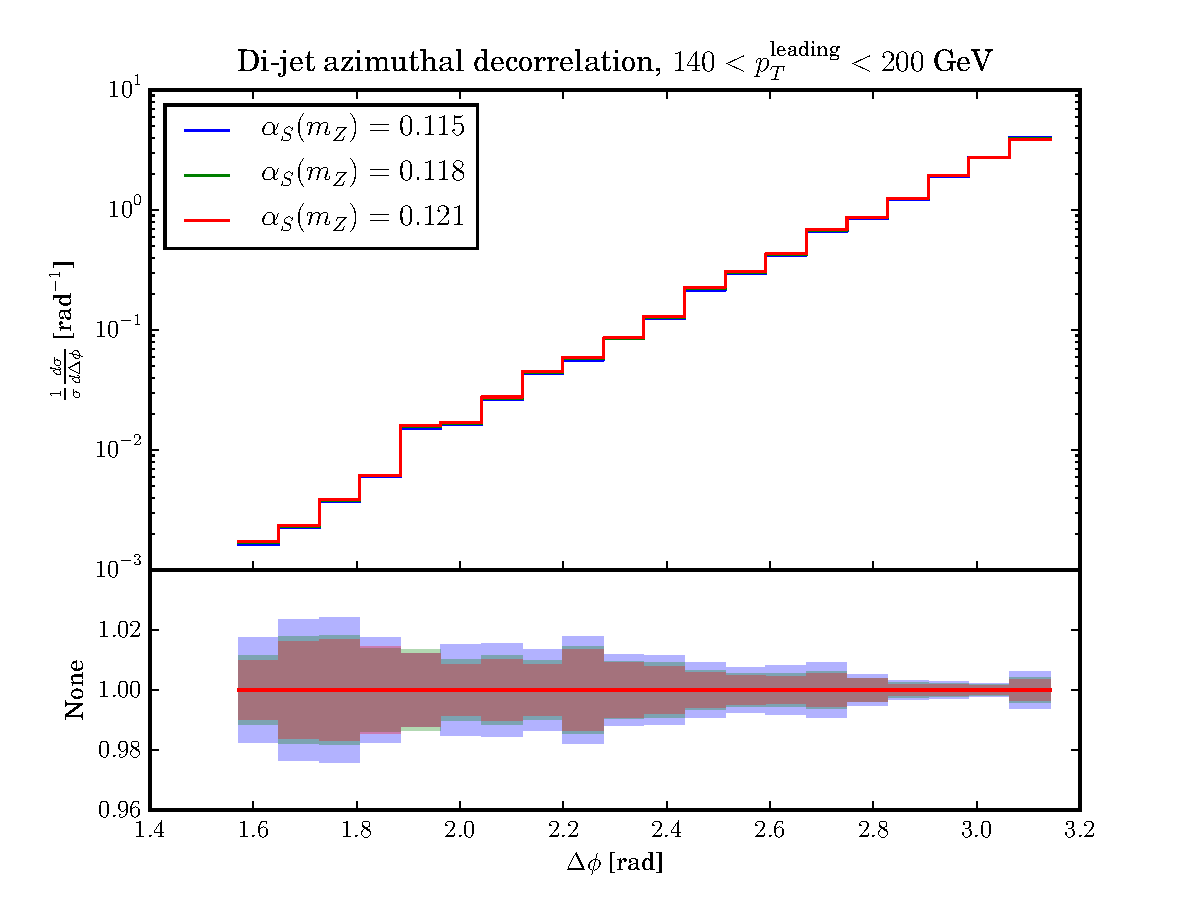
\includegraphics[width=0.49\textwidth]{d03-x01-y01_PDF-errors}
    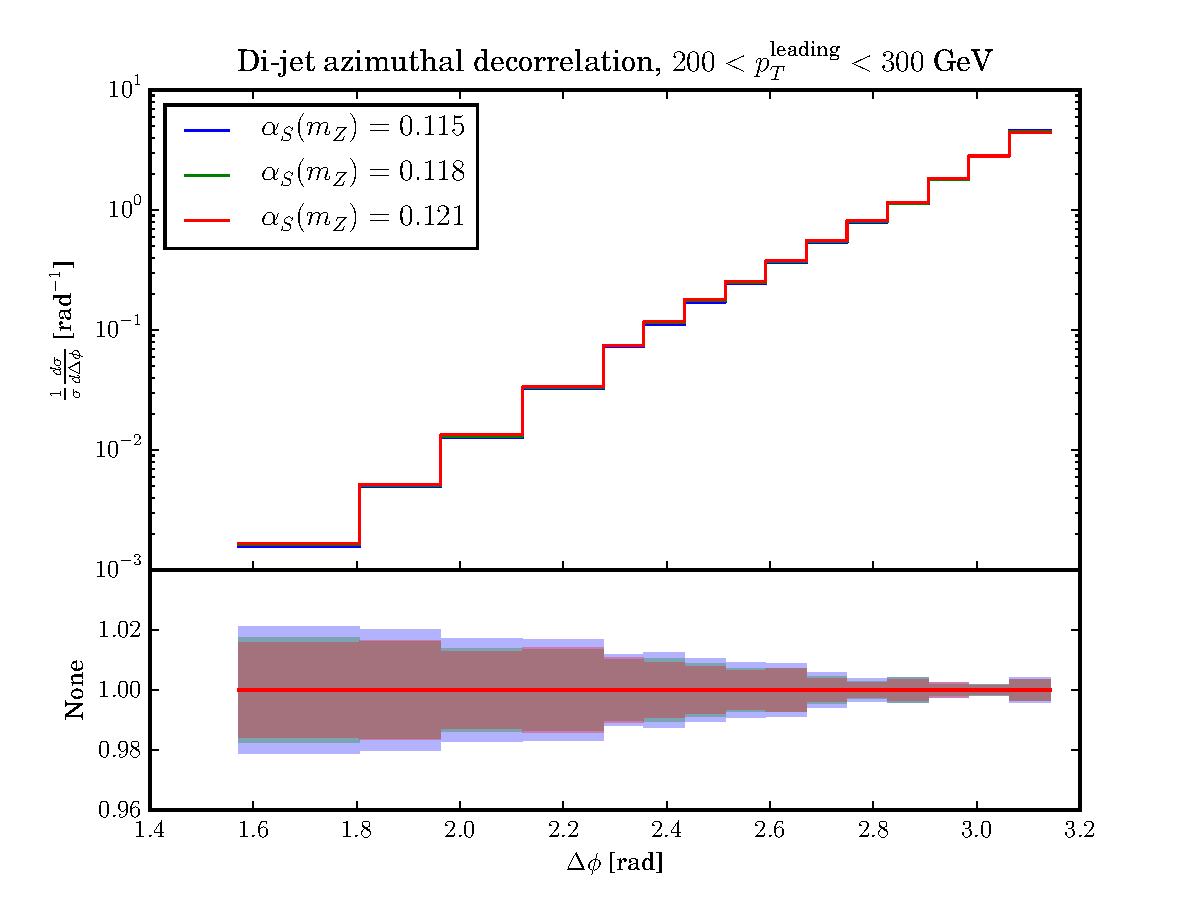
\includegraphics[width=0.49\textwidth]{d04-x01-y01_PDF-errors}
    \caption{PDF errors for the different $\alphas(m_Z)$ values
    in MCatNLO calculations.
    The errors are all of a similar shape, but for $\alphas(m_Z)=0.115$,
    the magnitude of the errors is about \SI{50}{\percent} larger.
    All variations have been calculated with a reweighting,
    where only the hardest emissions is included in the reweighting.}
    \label{fig:pdferrors}
\end{figure}
\section{Fit methodology and result}
Summarise the considerations for the \alphas fit.


\section{Reweighted Sudakov Veto Algorithm}
For convenience we reproduce the algorithm and the proof of the (reweighted)
Sudakov Veto Algorithm (SVA), in a similar way as
in~\cite{Hoeche:2009xc,Lonnblad:2012hz}.  Its purpose is to reuse the splitting
scales $\tvar$ determined by the normal SVA for a single Sudakov form factor
$\Delta$ with splitting kernel $f(\tvar)$
\begin{equation}
  \label{eq:sva_sudakov}
  \begin{split}
      \Delta_f(\tvar_2,\tvar_1)
    \,=\;\exp\left(-\int_{\tvar_2}^{\tvar_1}
         \diff \tvar\;
         f(\tvar)
         \right)\;,
  \end{split}
\end{equation}
in order predict observables for modified splitting kernels $h(\tvar)$.  To
keep the notation clean, we denote with $f(\tvar)$ the splitting kernels with
all kinematic variables except for the splitting scale itself integrated.

The error of using the same splitting scales for a different $h$ is compensated
by applying a weight for each trial emission within the SVA as follows:

\begin{enumerate}
    \item Start with $i=0$, a starting scale $\tvar_0$ and a weight $w=1$.
    \item Add 1 to $i$ and select $\tvar_i = G^{-1}\left(G(\tvar_{i-1}) - \log
        R \right)$ with the random number $R$, where $g$ is the integrable
        overestimate of the splitting kernel $f$ and $G$ its primitive.
        \label{sva:draw_t}
    \item Draw another random number $R'$; if $f(\tvar_i)/g(\tvar_i) \leq R'$,
    the trial emission is vetoed. In this case, multiply $w$ with 
    \begin{equation*}
        q'(\tvar_i) \equiv \frac{g(\tvar_i) - h(\tvar_i)}%
        {g(\tvar_i) - f(\tvar_i)}
    \end{equation*}
    and return to step \ref{sva:draw_t}.
    \item Otherwise, accept $\tvar_i$ as the first splitting scale below
        $\tvar_0$ and multiply $w$ with
    \begin{equation*}
        q(\tvar_i) \equiv \frac{h(\tvar_i)}{f(\tvar_i)}\;.
    \end{equation*}
\end{enumerate}

To prove that this algorithm produces the right splitting scale distribution
when the weight factors $q$ and $q'$ are applied, we first consider the
probabilities $\mathcal{P}_n(\tvar_0, \tvar)$ for accepting $\tvar$ as the first
splitting scale below $\tvar_0$ after $n$ vetoed trial emissions. If no trial
emission had been rejected, we obtain
\begin{equation}
    \label{eq:sva_p0}
    \mathcal{P}_0(\tvar_0, \tvar)
    = \mathcal{P}_g(\tvar_0, \tvar) \, \frac{f(\tvar)}{g(\tvar)} \, q(\tvar)\;.
\end{equation}
The first factor on the right hand side is defined as the probability that the
first emission below a starting scale $\tvar_0$ is at $\tvar$ when the
splitting kernel is $g$.  This probability is directly connected to the Sudakov
form factor, i.e. the no-emission probability between two scales:
\begin{equation}
    \mathcal{P}_g(\tvar_0, \tvar)
    = - \frac{\diff \Delta_g(\tvar_0, \tvar)}{\diff \tvar}
    = \Delta_g(\tvar_0, \tvar)\,g(\tvar)\;.
\end{equation}
The second factor on the RHS of~\eqref{eq:sva_p0} is the probability that the
SVA accepts $\tvar$, and the third one is the weight we apply for an accepted
emission. Inserting $\mathcal{P}_g$ and $q$ yields
\begin{equation}
    \mathcal{P}_0(\tvar_0, \tvar)
    = \Delta_g(\tvar_0, \tvar)\,h(\tvar_0, \tvar)\;.
\end{equation}

If exactly one emission has been rejected by the SVA by some intermediate scale
$\tvar_1$, we find
\begin{align}
    \mathcal{P}_1(\tvar_0, \tvar) &=
    \int_{\tvar_0}^{\tvar}\diff\tvar_1 \,
    \mathcal{P}_g(\tvar_0, \tvar_1) \,
    \left(1-\frac{f(\tvar_1)}{g(\tvar_1)}\right) \,
    q'(\tvar_1) \,
    \mathcal{P}_g(\tvar_1, \tvar) \,
    \frac{f(\tvar)}{g(\tvar)} \, q(\tvar) \\
    &=
    \mathcal{P}_0(\tvar_0, \tvar) \,
    \int_{\tvar_0}^{\tvar}\diff\tvar_1 \,
    \left(g(\tvar_1) - h(\tvar_1)\right)\;,
\end{align}
where we used
$\Delta(\tvar_0, \tvar_1)\Delta(\tvar_1,\tvar)=\Delta(\tvar_0,\tvar)$,
and had to put in the rejection probability $(1-f/g)$ and the rejection
weight~$q'$.

If exactly two emission have been rejected at intermediate scales $\tvar_1$ and
$\tvar_2$, we have
\begin{align}
    \mathcal{P}_2(\tvar_0, \tvar) &=
    \mathcal{P}_0(\tvar)\,
    \int_{\tvar_0}^{\tvar_1} \diff \tvar_1 \,
    \left(g(\tvar_1) - h(\tvar_1)\right)\,
    \int_{\tvar_1}^{\tvar} \diff \tvar_2 \,
    \left(g(\tvar_2) - h(\tvar_2)\right) \\
    &=
    \mathcal{P}_0(\tvar_0, \tvar) \,
    \frac{1}{2} \,
    \left[ \int_{\tvar_0}^{\tvar}\diff\tvar' \,
    \left(g(\tvar') - h(\tvar')\right)
    \right]^2\;,
\end{align}
where we extend the triangular integration area in the first line to a square
one to decouple the integrals. This is balanced by the factor 1/2.  This
pattern generalises to
\begin{equation}
    \mathcal{P}_n(\tvar_0, \tvar) =
    \mathcal{P}_0(\tvar_0, \tvar)\,
    \frac{1}{n!}\,
    \left[ \int_{\tvar_0}^{\tvar}\diff\tvar' \,
    \left(g(\tvar') - h(\tvar')\right)
    \right]^n\;.
\end{equation}

Because we are not interested in the number of rejections the SVA uses
internally, we have to sum over this number to get the actual distribution of
the (reweighted) SVA:
\begin{align}
    \mathcal{P}(\tvar_0, \tvar) &=
    \sum_{n=0}^\infty \mathcal{P}_n(\tvar_0, \tvar) \\
    &=
    \mathcal{P}_0(\tvar_0, \tvar)\,
    \sum_{n=0}^\infty
    \frac{1}{n!}\,
    \left[ \int_{\tvar_0}^{\tvar}\diff\tvar' \,
    \left(g(\tvar') - h(\tvar')\right)
    \right]^n \\
    &=
    \mathcal{P}_0(\tvar_0, \tvar)\,
    \exp\left\{
    \int_{\tvar_0}^{\tvar}\diff\tvar' \,
    \left(g(\tvar') - h(\tvar')\right)
    \right\} \\
    &=
    \Delta_h(\tvar_0, \tvar) \, h(\tvar) \\
    &=
    \mathcal{P}_h(\tvar_0, \tvar)\;,
\end{align}
which proves that the distribution for the splitting kernel $h$ is generated by
the reweighted SVA.

Note that the weights $q$ and $q'$ are exactly the factors by which the
acceptance and the veto probabilities are modified, if one would have used $h$
instead of $f$ in the first place.  This is obvious for the acceptance weight
$q$. For $q'$, a few lines of algebra is involved:
\begin{align}
    P_\text{veto}
    = 1 - P_\text{accept}
    &\to 1 - q P_\text{accept} \\
    &= \frac{1-q P_\text{accept}}{P_\text{veto}} \, P_\text{veto} \\
    &= \frac{1-q P_\text{accept}}{1-P_\text{accept}} \, P_\text{veto} \\
    &= \frac{1 - h/g}{1 - f/g} \, P_\text{veto} \\
    &= \frac{g - h}{g - f} \, P_\text{veto} = q' \, P_\text{veto}\;.
\end{align}

\bibliography{refs}
\bibliographystyle{plain}
\end{document}
